\section{Introduction}\label{sec:introduction}

\begin{quote}
\textbf{In plain words.} Every camera we use records light. Light is stopped by
walls, by rock and by the body of the Sun. Gravity is not stopped by anything.
This paper asks what a camera would show if it recorded gravity instead of
light.

One instrument already records gravity in this way.
\textbf{\href{https://en.wikipedia.org/wiki/LIGO}{LIGO}} is an observatory with
two arms, each four kilometres long. It detects
\textbf{\href{https://en.wikipedia.org/wiki/Gravitational_wave}{gravitational
waves}}: ripples in space that moving masses send out, and that stretch and
squeeze everything they pass through. LIGO gives one number at each moment, so
in the language of photography it is a camera with a single pixel. This paper
imagines a camera in which every pixel is such a detector, made as small and as
sensitive as we like. It then asks what picture that camera would give of an
ordinary scene, such as a room, a street or the ground under our feet.

Physics that is already well tested answers this question. Gravity is weak
everywhere except close to black holes and neutron stars. Where gravity is
weak, Einstein's theory of gravity becomes much simpler, because the gravity of
separate masses simply adds up. This simpler form of the theory is called
\textbf{\href{https://en.wikipedia.org/wiki/Linearized_gravity}{linearized
gravity}}. The camera does not respond to colour or brightness. It responds
only to where mass and energy are, to how they move, and to the pressure and
tension inside matter, which in Einstein's theory also produce gravity.

The camera can see in three different ways.
\begin{itemize}
\item \textbf{By the pull of nearby masses.} Close to an object, the camera
feels the object's gravity directly. It therefore sees the mass itself, and
walls do not block the view. The picture is blurred, however, and a better
detector sharpens it only very slowly. For example, a detector a thousand times
more sensitive narrows the blur only from about $24^\circ$ to about $14^\circ$.
(A blur of $24^\circ$ is roughly the width of an outstretched hand held at
arm's length.)
\item \textbf{By the gravitational waves of moving objects.} A spinning or
orbiting object sends out waves that are far longer than the object itself. A
wave cannot show details smaller than its own wavelength, so the camera sees
such an object as a single point, with no shape.
\item \textbf{By the gravitational glow of warm matter.} Heat makes atoms
jiggle, and jiggling masses send out very weak gravitational waves. These waves
are as short as infrared light, so in principle they could give pictures as
sharp as those of an infrared camera. Matter hardly absorbs them, so solid
matter is transparent to them. At midnight, a camera pointed at the ground
would see the Sun's core shining through the Earth. The glow is extremely
faint, however. It arrives as
\textbf{\href{https://en.wikipedia.org/wiki/Graviton}{gravitons}}, the smallest
possible packets of gravitational-wave energy, just as light arrives as
photons. So few gravitons arrive that a whole lifetime of collecting would give
only a very coarse picture.
\end{itemize}

No lens or mirror can be made for gravitational waves, because matter barely
affects them. The camera must therefore compute its pictures from what its
pixels record. A single pixel also turns out to measure much more than one
would expect. For example, it can find its own velocity.

The last part of the paper asks how much the gravity outside a body reveals
about its inside. Newton's
\textbf{\href{https://en.wikipedia.org/wiki/Shell_theorem}{shell theorem}} says
that a hollow shell and a solid ball of the same mass pull in exactly the same
way on everything outside them. For black holes, the
\textbf{\href{https://en.wikipedia.org/wiki/No-hair_theorem}{no-hair theorem}}
says that the gravity outside shows only the mass, the spin and the electric
charge. The paper's main result is that the gravity of an ordinary body can
reveal far more than Newton's theorem suggests. A single snapshot of the body's
gravity shows only certain overall features of how its mass is arranged. A
second mass that flies past the body, however, sets the body's parts moving and
leaves some energy in them. The passing mass loses that energy from its own
motion, so it ends up slightly slower. How much slower depends on where the
body's mass lies. The losses along many different paths that miss the body give
the body's density everywhere inside. A black hole, tested in the same ways,
reveals only its mass, its spin and its temperature.

Most of the effects in this paper are far too small for any instrument we could
build. The paper is a thought experiment about what gravity carries in
principle.
\end{quote}

Gravitational waves were first detected in 2015 by LIGO \cite{LIGO2016}, an instrument four
kilometres long that reports a single number at each instant. In the language
of photography it is a camera with one pixel. This paper takes that language
seriously. We suppose that such detectors could be made as small and as
sensitive as we please, place one at every pixel of a sensor, and ask what
picture results when the sensor is pointed at an ordinary scene: a room, a
street, the ground beneath our feet.

The question has an answer because gravity is simple where it is weak. Every
form of matter and energy produces it, in proportion to its energy (and, for
fast motion and for light, its momentum and stress too), whatever it is made
of, and nothing shields it. The weakness that makes gravity so hard to detect makes a
gravitational camera easy to reason about: we need only the linear theory, and
the stress and motion of the matter in view.

Our results are these.
\begin{itemize}
\item A pixel measures the \emph{tidal field}, ten numbers at each point
(Section~\ref{sec:pixel}). One component of it, which is what an interferometer reads, cannot tell a
passing wave from the pull of a nearby object, and for everyday scenes the pull
dominates.
\item What the camera sees falls into three regimes, set by how far the source
is compared with the wavelength it would radiate (Section~\ref{sec:regimes}).
\item In the near field the camera sees mass itself, moving or still, through
any obstacle. Its blur is a fixed fraction of the distance, and improves only
with the logarithm of the sensitivity, for clocks and accelerometers as much as
for tidal pixels; but mass is never negative, and a scene of a few bodies is
measured far more sharply than it can be drawn. A body's steady pull hides its
interior; its thermal tremor, at a known temperature, reveals it, and a tide
applied from outside does the same at any temperature (Section~\ref{sec:near-field}).
\item In the waves radiated by moving bodies, a compact body moving slowly is
smaller than its own wavelength and appears as a point
(Section~\ref{sec:waves}).
\item In thermal radiation the camera can be as sharp as an infrared camera.
Matter is transparent, and glows in proportion to its internal friction and a
power of its temperature, up to a limit that a sum rule sets for every material
(Section~\ref{sec:thermal}).
\item Matter cannot act as a useful lens, a mirror or a screen for gravitational
waves, so the image must be computed from what the pixels record
(Section~\ref{sec:no-lens}).
\item One pixel measures far more than a sensor of light at a point, and a few
pixels more still (Section~\ref{sec:one-pixel}). A pixel's ten numbers are four
invariants, the orientation of the field and the velocity of its rest frame, so
it reads its own velocity through an unknown scene and detects motion within it
whatever its own. It tells whether its field could come from a single round
body or a single wave, reads a moving body's position, velocity and mass exactly at any
speed, separates up to four waves crossing it (a count that one theorem gives
for a field of any spin), ranges a wave source, sees moving
bodies where they are now rather than where they were, and reads the speed and
all six polarizations of a wave in one reading. Its magnetic part separates a
wave from the pull of nearby objects at a fixed cost in noise, and supplies the
one scale the electric part lacks, so a single pixel ranges a moving mass; a
few pixels side by side measure distance from how the field varies.
\item The expected number of gravitons that arrive sets what there is to be
seen: a first image, with its budget, and the reason why nothing made of
matter could catch it (Section~\ref{sec:first-image}).
Section~\ref{sec:affordances} lists what the camera can do that light cannot.
\item On the scale of the sky (Section~\ref{sec:vistas}): the field of two
black holes in orbit changes, at a sixth of their wavelength, from the pull of
two bodies to the waves of one; a spherical explosion sends out no waves,
and a lopsided one leaves space permanently stretched;
the Galaxy's centre, hidden from light by dust, is the brightest part of the
millihertz sky; and if the Big Bang was ever hot enough to make gravitons in
equilibrium, the whole sky glows at $0.905\,\mathrm{K}$, shares the large
spots of the microwave background, and has nothing dark on it but black
holes.
\item What the field outside a body determines of its interior is one
subject, gravitational hair (Sections~\ref{sec:hair} to~\ref{sec:holography}). The field at one time
gives the harmonic part of the body's mass and no more; the field at two times
gives all of it, through the same logarithm; and a black hole at rest yields seven
numbers to the first measurement and only its temperature to the second; its
response to a changing quadrupolar tide has the inertia of a shell of its own
mass just outside its horizon, and its responses to the first three tides
together that of no distribution of positive mass. The ambiguity is that of Newton's shell
theorem, and it holds only to first order in the mass of whatever feels the
field. The second measurement can be a tide applied from outside, followed by
a weighing, or a single mass that flies past the body: the energy it leaves
behind is taken from its own motion, and the amounts lost on the paths that
miss the body give all of the body's density. This is what remains in
classical physics of the holography argued for quantum gravity.
How much is reached depends on the tide. Tides of degree up to $m$ give $m$
radial moments of the density in every angular sector and no more, so that
there are bodies which no quadrupolar tide tells apart to leading order and an octupolar tide
does; two tides applied in either order give the flow within the body; and
an impulsive gravitational wave reads, at any speed, the energy that crosses
each point of its front.
\end{itemize}

Figure~\ref{fig:sun-at-midnight} shows where this leads. An observer stands on
the night side of the Earth and looks down. In light there is only dark ground.
In thermal gravitational radiation the planet is a set of glowing shells, and
beyond it, shining straight through, is the core of the Sun.

\begin{figure*}
\centering
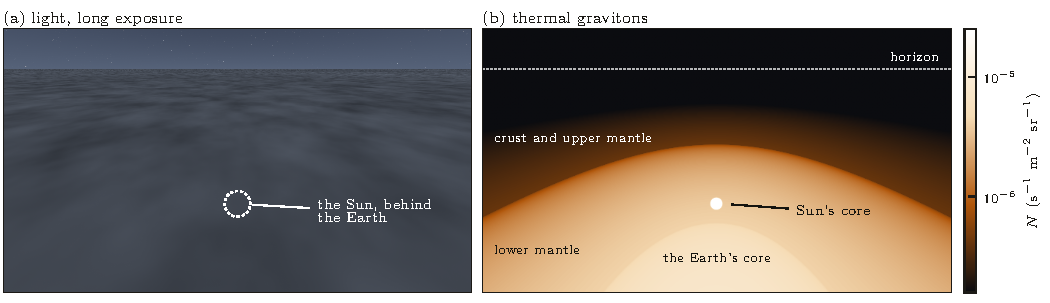
\includegraphics[width=\textwidth]{figures/sun-at-midnight.pdf}
\caption{The Sun at midnight, computed. An observer at latitude
$40^\circ$ north looks north and down, $33^\circ$ below the horizon, at local
midnight, with the same camera, $86^\circ$ from top to bottom, in both panels. (a) Ordinary light, exposed long enough to show the ground; the dotted
circle marks where the Sun lies, behind the planet. (b) Thermal gravitational
radiation: the expected number radiance $N(\hat n)$ of Eq.~\eqref{eq:column},
on a logarithmic scale. The ground is transparent. Lines of sight just below
the horizon cross only the crust and upper mantle and are faint; steeper ones
cross the hotter lower mantle, and those within $33^\circ$ of straight down,
at the foot of the picture, the core (Fig.~\ref{fig:earth-glow}). The Sun's core, $50^\circ$ below the horizon, is
smaller than a pixel; its flux, under one graviton per square metre per second,
is spread over a spot a few pixels across, far brighter than the top of the
scale. Section~\ref{sec:first-image} gives the model and its
assumptions.}\label{fig:sun-at-midnight}
\end{figure*}

\paragraph{What is already known.} The ingredients exist separately. Gravity
sensors already map buried structures by their pull \cite{Stray2022}; small
gravimeters are being made cheap enough to be set out as the pixels of an
imager \cite{Middlemiss2016,Prasad2021}, and a patent calls an array of them a
gravity camera \cite{JordanHowell2021}. The designers of LIGO worked out how strongly a walking
person disturbs it \cite{ThorneWinstein1999}, and seismologists have recorded
the gravitational signal of an earthquake arriving before the shaking
\cite{Vallee2017}. Gravity gradiometry has been proposed for imaging the contents
of cargo containers \cite{Kirkendall2007} and for locating objects under water
\cite{WuTian2010}. Networks of pulsars are analyzed as imaging telescopes for
gravitational waves from the distant universe \cite{BoylePen2012}, the
gravitational radiation of the Sun has been calculated
\cite{GarciaCelyRingwald2025,Steane2024}, and the tidal field has been
visualized around black holes and simple sources \cite{Nichols2011}. Much of
the algebra of a single reading is known in other forms: the frame in which the
electric and magnetic parts share their axes, the principal observer, has been
built from the curvature's invariants
\cite{CostaWyllemanNatario2021,WyllemanCostaNatario2021}; the
cross product of the two parts is the curvature's super-Poynting vector
\cite{MaartensBassett1998}; curvature can be measured operationally with test
bodies and clocks \cite{ObukhovPuetzfeld2019}; and the
polarization of a harmonic wave, as a detector of both parts would record it at
one place, has been drawn as four points on the sky \cite{Bruno2019}. What we
add is a single account of what an ideal observer of the tidal field would
record of ordinary surroundings, followed from the near field to the radiation
field and the thermal glow, with the limits of each regime stated.
